% Created by tikzDevice version 0.12.3.1 on 2022-11-29 21:13:36
% !TEX encoding = UTF-8 Unicode
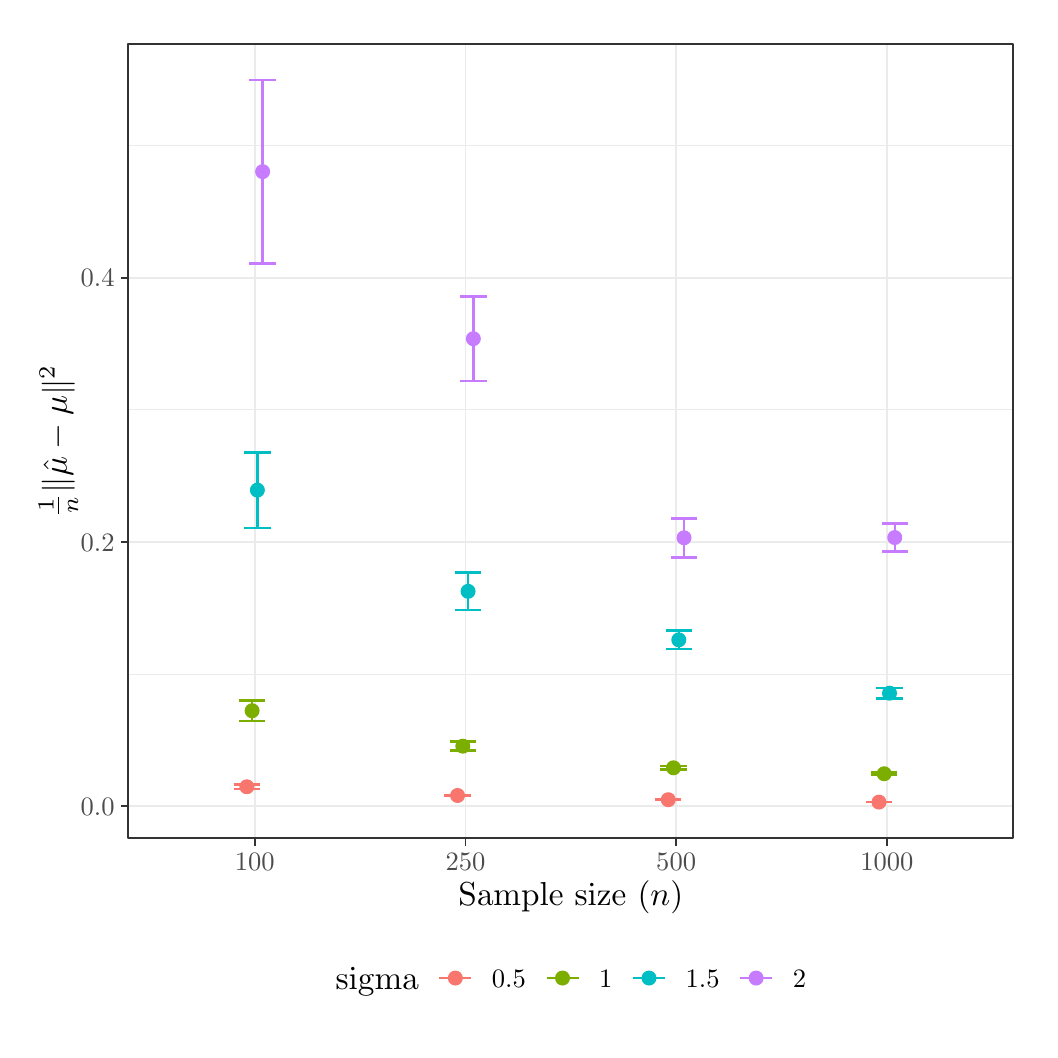
\begin{tikzpicture}[x=1pt,y=1pt]
\definecolor{fillColor}{RGB}{255,255,255}
\begin{scope}
\definecolor{drawColor}{RGB}{255,255,255}
\definecolor{fillColor}{RGB}{255,255,255}

\path[draw=drawColor,line width= 0.6pt,line join=round,line cap=round,fill=fillColor] (  0.00,  0.00) rectangle (361.35,361.35);
\end{scope}
\begin{scope}
\definecolor{fillColor}{RGB}{255,255,255}

\path[fill=fillColor] ( 36.06, 68.73) rectangle (355.85,355.85);
\definecolor{drawColor}{gray}{0.92}

\path[draw=drawColor,line width= 0.3pt,line join=round] ( 36.06,128.05) --
	(355.85,128.05);

\path[draw=drawColor,line width= 0.3pt,line join=round] ( 36.06,223.55) --
	(355.85,223.55);

\path[draw=drawColor,line width= 0.3pt,line join=round] ( 36.06,319.05) --
	(355.85,319.05);

\path[draw=drawColor,line width= 0.6pt,line join=round] ( 36.06, 80.30) --
	(355.85, 80.30);

\path[draw=drawColor,line width= 0.6pt,line join=round] ( 36.06,175.80) --
	(355.85,175.80);

\path[draw=drawColor,line width= 0.6pt,line join=round] ( 36.06,271.30) --
	(355.85,271.30);

\path[draw=drawColor,line width= 0.6pt,line join=round] ( 81.75, 68.73) --
	( 81.75,355.85);

\path[draw=drawColor,line width= 0.6pt,line join=round] (157.89, 68.73) --
	(157.89,355.85);

\path[draw=drawColor,line width= 0.6pt,line join=round] (234.03, 68.73) --
	(234.03,355.85);

\path[draw=drawColor,line width= 0.6pt,line join=round] (310.17, 68.73) --
	(310.17,355.85);
\definecolor{drawColor}{RGB}{248,118,109}

\path[draw=drawColor,line width= 0.9pt,line join=round] ( 74.13, 88.12) --
	( 83.65, 88.12);

\path[draw=drawColor,line width= 0.9pt,line join=round] ( 78.89, 88.12) --
	( 78.89, 86.58);

\path[draw=drawColor,line width= 0.9pt,line join=round] ( 74.13, 86.58) --
	( 83.65, 86.58);
\definecolor{drawColor}{RGB}{124,174,0}

\path[draw=drawColor,line width= 0.9pt,line join=round] ( 76.03,118.60) --
	( 85.55,118.60);

\path[draw=drawColor,line width= 0.9pt,line join=round] ( 80.79,118.60) --
	( 80.79,111.05);

\path[draw=drawColor,line width= 0.9pt,line join=round] ( 76.03,111.05) --
	( 85.55,111.05);
\definecolor{drawColor}{RGB}{0,191,196}

\path[draw=drawColor,line width= 0.9pt,line join=round] ( 77.94,208.18) --
	( 87.46,208.18);

\path[draw=drawColor,line width= 0.9pt,line join=round] ( 82.70,208.18) --
	( 82.70,180.93);

\path[draw=drawColor,line width= 0.9pt,line join=round] ( 77.94,180.93) --
	( 87.46,180.93);
\definecolor{drawColor}{RGB}{199,124,255}

\path[draw=drawColor,line width= 0.9pt,line join=round] ( 79.84,342.80) --
	( 89.36,342.80);

\path[draw=drawColor,line width= 0.9pt,line join=round] ( 84.60,342.80) --
	( 84.60,276.44);

\path[draw=drawColor,line width= 0.9pt,line join=round] ( 79.84,276.44) --
	( 89.36,276.44);
\definecolor{drawColor}{RGB}{248,118,109}

\path[draw=drawColor,line width= 0.9pt,line join=round] (150.27, 84.39) --
	(159.79, 84.39);

\path[draw=drawColor,line width= 0.9pt,line join=round] (155.03, 84.39) --
	(155.03, 84.01);

\path[draw=drawColor,line width= 0.9pt,line join=round] (150.27, 84.01) --
	(159.79, 84.01);
\definecolor{drawColor}{RGB}{124,174,0}

\path[draw=drawColor,line width= 0.9pt,line join=round] (152.17,103.66) --
	(161.69,103.66);

\path[draw=drawColor,line width= 0.9pt,line join=round] (156.93,103.66) --
	(156.93,100.38);

\path[draw=drawColor,line width= 0.9pt,line join=round] (152.17,100.38) --
	(161.69,100.38);
\definecolor{drawColor}{RGB}{0,191,196}

\path[draw=drawColor,line width= 0.9pt,line join=round] (154.08,164.69) --
	(163.60,164.69);

\path[draw=drawColor,line width= 0.9pt,line join=round] (158.84,164.69) --
	(158.84,151.26);

\path[draw=drawColor,line width= 0.9pt,line join=round] (154.08,151.26) --
	(163.60,151.26);
\definecolor{drawColor}{RGB}{199,124,255}

\path[draw=drawColor,line width= 0.9pt,line join=round] (155.98,264.50) --
	(165.50,264.50);

\path[draw=drawColor,line width= 0.9pt,line join=round] (160.74,264.50) --
	(160.74,234.01);

\path[draw=drawColor,line width= 0.9pt,line join=round] (155.98,234.01) --
	(165.50,234.01);
\definecolor{drawColor}{RGB}{248,118,109}

\path[draw=drawColor,line width= 0.9pt,line join=round] (226.41, 82.77) --
	(235.93, 82.77);

\path[draw=drawColor,line width= 0.9pt,line join=round] (231.17, 82.77) --
	(231.17, 82.57);

\path[draw=drawColor,line width= 0.9pt,line join=round] (226.41, 82.57) --
	(235.93, 82.57);
\definecolor{drawColor}{RGB}{124,174,0}

\path[draw=drawColor,line width= 0.9pt,line join=round] (228.32, 94.80) --
	(237.83, 94.80);

\path[draw=drawColor,line width= 0.9pt,line join=round] (233.07, 94.80) --
	(233.07, 93.60);

\path[draw=drawColor,line width= 0.9pt,line join=round] (228.32, 93.60) --
	(237.83, 93.60);
\definecolor{drawColor}{RGB}{0,191,196}

\path[draw=drawColor,line width= 0.9pt,line join=round] (230.22,143.85) --
	(239.74,143.85);

\path[draw=drawColor,line width= 0.9pt,line join=round] (234.98,143.85) --
	(234.98,137.04);

\path[draw=drawColor,line width= 0.9pt,line join=round] (230.22,137.04) --
	(239.74,137.04);
\definecolor{drawColor}{RGB}{199,124,255}

\path[draw=drawColor,line width= 0.9pt,line join=round] (232.12,184.36) --
	(241.64,184.36);

\path[draw=drawColor,line width= 0.9pt,line join=round] (236.88,184.36) --
	(236.88,170.28);

\path[draw=drawColor,line width= 0.9pt,line join=round] (232.12,170.28) --
	(241.64,170.28);
\definecolor{drawColor}{RGB}{248,118,109}

\path[draw=drawColor,line width= 0.9pt,line join=round] (302.55, 81.84) --
	(312.07, 81.84);

\path[draw=drawColor,line width= 0.9pt,line join=round] (307.31, 81.84) --
	(307.31, 81.78);

\path[draw=drawColor,line width= 0.9pt,line join=round] (302.55, 81.78) --
	(312.07, 81.78);
\definecolor{drawColor}{RGB}{124,174,0}

\path[draw=drawColor,line width= 0.9pt,line join=round] (304.46, 92.52) --
	(313.97, 92.52);

\path[draw=drawColor,line width= 0.9pt,line join=round] (309.21, 92.52) --
	(309.21, 91.58);

\path[draw=drawColor,line width= 0.9pt,line join=round] (304.46, 91.58) --
	(313.97, 91.58);
\definecolor{drawColor}{RGB}{0,191,196}

\path[draw=drawColor,line width= 0.9pt,line join=round] (306.36,123.02) --
	(315.88,123.02);

\path[draw=drawColor,line width= 0.9pt,line join=round] (311.12,123.02) --
	(311.12,119.32);

\path[draw=drawColor,line width= 0.9pt,line join=round] (306.36,119.32) --
	(315.88,119.32);
\definecolor{drawColor}{RGB}{199,124,255}

\path[draw=drawColor,line width= 0.9pt,line join=round] (308.26,182.52) --
	(317.78,182.52);

\path[draw=drawColor,line width= 0.9pt,line join=round] (313.02,182.52) --
	(313.02,172.30);

\path[draw=drawColor,line width= 0.9pt,line join=round] (308.26,172.30) --
	(317.78,172.30);
\definecolor{drawColor}{RGB}{248,118,109}
\definecolor{fillColor}{RGB}{248,118,109}

\path[draw=drawColor,line width= 0.4pt,line join=round,line cap=round,fill=fillColor] ( 78.89, 87.35) circle (  2.50);
\definecolor{drawColor}{RGB}{124,174,0}
\definecolor{fillColor}{RGB}{124,174,0}

\path[draw=drawColor,line width= 0.4pt,line join=round,line cap=round,fill=fillColor] ( 80.79,114.82) circle (  2.50);
\definecolor{drawColor}{RGB}{0,191,196}
\definecolor{fillColor}{RGB}{0,191,196}

\path[draw=drawColor,line width= 0.4pt,line join=round,line cap=round,fill=fillColor] ( 82.70,194.55) circle (  2.50);
\definecolor{drawColor}{RGB}{199,124,255}
\definecolor{fillColor}{RGB}{199,124,255}

\path[draw=drawColor,line width= 0.4pt,line join=round,line cap=round,fill=fillColor] ( 84.60,309.62) circle (  2.50);
\definecolor{drawColor}{RGB}{248,118,109}
\definecolor{fillColor}{RGB}{248,118,109}

\path[draw=drawColor,line width= 0.4pt,line join=round,line cap=round,fill=fillColor] (155.03, 84.20) circle (  2.50);
\definecolor{drawColor}{RGB}{124,174,0}
\definecolor{fillColor}{RGB}{124,174,0}

\path[draw=drawColor,line width= 0.4pt,line join=round,line cap=round,fill=fillColor] (156.93,102.02) circle (  2.50);
\definecolor{drawColor}{RGB}{0,191,196}
\definecolor{fillColor}{RGB}{0,191,196}

\path[draw=drawColor,line width= 0.4pt,line join=round,line cap=round,fill=fillColor] (158.84,157.97) circle (  2.50);
\definecolor{drawColor}{RGB}{199,124,255}
\definecolor{fillColor}{RGB}{199,124,255}

\path[draw=drawColor,line width= 0.4pt,line join=round,line cap=round,fill=fillColor] (160.74,249.26) circle (  2.50);
\definecolor{drawColor}{RGB}{248,118,109}
\definecolor{fillColor}{RGB}{248,118,109}

\path[draw=drawColor,line width= 0.4pt,line join=round,line cap=round,fill=fillColor] (231.17, 82.67) circle (  2.50);
\definecolor{drawColor}{RGB}{124,174,0}
\definecolor{fillColor}{RGB}{124,174,0}

\path[draw=drawColor,line width= 0.4pt,line join=round,line cap=round,fill=fillColor] (233.07, 94.20) circle (  2.50);
\definecolor{drawColor}{RGB}{0,191,196}
\definecolor{fillColor}{RGB}{0,191,196}

\path[draw=drawColor,line width= 0.4pt,line join=round,line cap=round,fill=fillColor] (234.98,140.44) circle (  2.50);
\definecolor{drawColor}{RGB}{199,124,255}
\definecolor{fillColor}{RGB}{199,124,255}

\path[draw=drawColor,line width= 0.4pt,line join=round,line cap=round,fill=fillColor] (236.88,177.32) circle (  2.50);
\definecolor{drawColor}{RGB}{248,118,109}
\definecolor{fillColor}{RGB}{248,118,109}

\path[draw=drawColor,line width= 0.4pt,line join=round,line cap=round,fill=fillColor] (307.31, 81.81) circle (  2.50);
\definecolor{drawColor}{RGB}{124,174,0}
\definecolor{fillColor}{RGB}{124,174,0}

\path[draw=drawColor,line width= 0.4pt,line join=round,line cap=round,fill=fillColor] (309.21, 92.05) circle (  2.50);
\definecolor{drawColor}{RGB}{0,191,196}
\definecolor{fillColor}{RGB}{0,191,196}

\path[draw=drawColor,line width= 0.4pt,line join=round,line cap=round,fill=fillColor] (311.12,121.17) circle (  2.50);
\definecolor{drawColor}{RGB}{199,124,255}
\definecolor{fillColor}{RGB}{199,124,255}

\path[draw=drawColor,line width= 0.4pt,line join=round,line cap=round,fill=fillColor] (313.02,177.41) circle (  2.50);
\definecolor{drawColor}{gray}{0.20}

\path[draw=drawColor,line width= 0.6pt,line join=round,line cap=round] ( 36.06, 68.73) rectangle (355.85,355.85);
\end{scope}
\begin{scope}
\definecolor{drawColor}{gray}{0.30}

\node[text=drawColor,anchor=base east,inner sep=0pt, outer sep=0pt, scale=  0.96] at ( 31.11, 76.99) {0.0};

\node[text=drawColor,anchor=base east,inner sep=0pt, outer sep=0pt, scale=  0.96] at ( 31.11,172.49) {0.2};

\node[text=drawColor,anchor=base east,inner sep=0pt, outer sep=0pt, scale=  0.96] at ( 31.11,268.00) {0.4};
\end{scope}
\begin{scope}
\definecolor{drawColor}{gray}{0.20}

\path[draw=drawColor,line width= 0.6pt,line join=round] ( 33.31, 80.30) --
	( 36.06, 80.30);

\path[draw=drawColor,line width= 0.6pt,line join=round] ( 33.31,175.80) --
	( 36.06,175.80);

\path[draw=drawColor,line width= 0.6pt,line join=round] ( 33.31,271.30) --
	( 36.06,271.30);
\end{scope}
\begin{scope}
\definecolor{drawColor}{gray}{0.20}

\path[draw=drawColor,line width= 0.6pt,line join=round] ( 81.75, 65.98) --
	( 81.75, 68.73);

\path[draw=drawColor,line width= 0.6pt,line join=round] (157.89, 65.98) --
	(157.89, 68.73);

\path[draw=drawColor,line width= 0.6pt,line join=round] (234.03, 65.98) --
	(234.03, 68.73);

\path[draw=drawColor,line width= 0.6pt,line join=round] (310.17, 65.98) --
	(310.17, 68.73);
\end{scope}
\begin{scope}
\definecolor{drawColor}{gray}{0.30}

\node[text=drawColor,anchor=base,inner sep=0pt, outer sep=0pt, scale=  0.96] at ( 81.75, 57.17) {100};

\node[text=drawColor,anchor=base,inner sep=0pt, outer sep=0pt, scale=  0.96] at (157.89, 57.17) {250};

\node[text=drawColor,anchor=base,inner sep=0pt, outer sep=0pt, scale=  0.96] at (234.03, 57.17) {500};

\node[text=drawColor,anchor=base,inner sep=0pt, outer sep=0pt, scale=  0.96] at (310.17, 57.17) {1000};
\end{scope}
\begin{scope}
\definecolor{drawColor}{RGB}{0,0,0}

\node[text=drawColor,anchor=base,inner sep=0pt, outer sep=0pt, scale=  1.20] at (195.96, 44.29) {Sample size $(n)$};
\end{scope}
\begin{scope}
\definecolor{drawColor}{RGB}{0,0,0}

\node[text=drawColor,rotate= 90.00,anchor=base,inner sep=0pt, outer sep=0pt, scale=  1.20] at ( 13.76,212.29) {$\frac{1}{n} \| \hat{\mu} - \mu \|^{2}$};
\end{scope}
\begin{scope}
\definecolor{fillColor}{RGB}{255,255,255}

\path[fill=fillColor] (105.46,  5.50) rectangle (286.46, 30.95);
\end{scope}
\begin{scope}
\definecolor{drawColor}{RGB}{0,0,0}

\node[text=drawColor,anchor=base west,inner sep=0pt, outer sep=0pt, scale=  1.20] at (110.96, 14.09) {sigma};
\end{scope}
\begin{scope}
\definecolor{fillColor}{RGB}{255,255,255}

\path[fill=fillColor] (147.01, 11.00) rectangle (161.47, 25.45);
\end{scope}
\begin{scope}
\definecolor{drawColor}{RGB}{248,118,109}

\path[draw=drawColor,line width= 0.9pt,line join=round] (148.46, 18.23) -- (160.02, 18.23);
\end{scope}
\begin{scope}
\definecolor{drawColor}{RGB}{248,118,109}

\path[draw=drawColor,line width= 0.6pt,line join=round] (148.46, 18.23) -- (160.02, 18.23);
\end{scope}
\begin{scope}
\definecolor{drawColor}{RGB}{248,118,109}
\definecolor{fillColor}{RGB}{248,118,109}

\path[draw=drawColor,line width= 0.4pt,line join=round,line cap=round,fill=fillColor] (154.24, 18.23) circle (  2.50);
\end{scope}
\begin{scope}
\definecolor{fillColor}{RGB}{255,255,255}

\path[fill=fillColor] (185.73, 11.00) rectangle (200.19, 25.45);
\end{scope}
\begin{scope}
\definecolor{drawColor}{RGB}{124,174,0}

\path[draw=drawColor,line width= 0.9pt,line join=round] (187.18, 18.23) -- (198.74, 18.23);
\end{scope}
\begin{scope}
\definecolor{drawColor}{RGB}{124,174,0}

\path[draw=drawColor,line width= 0.6pt,line join=round] (187.18, 18.23) -- (198.74, 18.23);
\end{scope}
\begin{scope}
\definecolor{drawColor}{RGB}{124,174,0}
\definecolor{fillColor}{RGB}{124,174,0}

\path[draw=drawColor,line width= 0.4pt,line join=round,line cap=round,fill=fillColor] (192.96, 18.23) circle (  2.50);
\end{scope}
\begin{scope}
\definecolor{fillColor}{RGB}{255,255,255}

\path[fill=fillColor] (216.99, 11.00) rectangle (231.44, 25.45);
\end{scope}
\begin{scope}
\definecolor{drawColor}{RGB}{0,191,196}

\path[draw=drawColor,line width= 0.9pt,line join=round] (218.43, 18.23) -- (229.99, 18.23);
\end{scope}
\begin{scope}
\definecolor{drawColor}{RGB}{0,191,196}

\path[draw=drawColor,line width= 0.6pt,line join=round] (218.43, 18.23) -- (229.99, 18.23);
\end{scope}
\begin{scope}
\definecolor{drawColor}{RGB}{0,191,196}
\definecolor{fillColor}{RGB}{0,191,196}

\path[draw=drawColor,line width= 0.4pt,line join=round,line cap=round,fill=fillColor] (224.21, 18.23) circle (  2.50);
\end{scope}
\begin{scope}
\definecolor{fillColor}{RGB}{255,255,255}

\path[fill=fillColor] (255.70, 11.00) rectangle (270.16, 25.45);
\end{scope}
\begin{scope}
\definecolor{drawColor}{RGB}{199,124,255}

\path[draw=drawColor,line width= 0.9pt,line join=round] (257.15, 18.23) -- (268.71, 18.23);
\end{scope}
\begin{scope}
\definecolor{drawColor}{RGB}{199,124,255}

\path[draw=drawColor,line width= 0.6pt,line join=round] (257.15, 18.23) -- (268.71, 18.23);
\end{scope}
\begin{scope}
\definecolor{drawColor}{RGB}{199,124,255}
\definecolor{fillColor}{RGB}{199,124,255}

\path[draw=drawColor,line width= 0.4pt,line join=round,line cap=round,fill=fillColor] (262.93, 18.23) circle (  2.50);
\end{scope}
\begin{scope}
\definecolor{drawColor}{RGB}{0,0,0}

\node[text=drawColor,anchor=base west,inner sep=0pt, outer sep=0pt, scale=  0.96] at (167.47, 14.92) {0.5};
\end{scope}
\begin{scope}
\definecolor{drawColor}{RGB}{0,0,0}

\node[text=drawColor,anchor=base west,inner sep=0pt, outer sep=0pt, scale=  0.96] at (206.19, 14.92) {1};
\end{scope}
\begin{scope}
\definecolor{drawColor}{RGB}{0,0,0}

\node[text=drawColor,anchor=base west,inner sep=0pt, outer sep=0pt, scale=  0.96] at (237.44, 14.92) {1.5};
\end{scope}
\begin{scope}
\definecolor{drawColor}{RGB}{0,0,0}

\node[text=drawColor,anchor=base west,inner sep=0pt, outer sep=0pt, scale=  0.96] at (276.16, 14.92) {2};
\end{scope}
\end{tikzpicture}
